\documentclass[]{article}
\usepackage{lmodern}
\usepackage{amssymb,amsmath}
\usepackage{ifxetex,ifluatex}
\usepackage{fixltx2e} % provides \textsubscript
\ifnum 0\ifxetex 1\fi\ifluatex 1\fi=0 % if pdftex
  \usepackage[T1]{fontenc}
  \usepackage[utf8]{inputenc}
\else % if luatex or xelatex
  \ifxetex
    \usepackage{mathspec}
  \else
    \usepackage{fontspec}
  \fi
  \defaultfontfeatures{Ligatures=TeX,Scale=MatchLowercase}
\fi
% use upquote if available, for straight quotes in verbatim environments
\IfFileExists{upquote.sty}{\usepackage{upquote}}{}
% use microtype if available
\IfFileExists{microtype.sty}{%
\usepackage{microtype}
\UseMicrotypeSet[protrusion]{basicmath} % disable protrusion for tt fonts
}{}
\usepackage[margin=1in]{geometry}
\usepackage{hyperref}
\hypersetup{unicode=true,
            pdftitle={Solving PDE's with Neural Networks},
            pdfauthor={Sigurd Hylin},
            pdfborder={0 0 0},
            breaklinks=true}
\urlstyle{same}  % don't use monospace font for urls
\usepackage{natbib}
\bibliographystyle{plainnat}
\usepackage{graphicx,grffile}
\makeatletter
\def\maxwidth{\ifdim\Gin@nat@width>\linewidth\linewidth\else\Gin@nat@width\fi}
\def\maxheight{\ifdim\Gin@nat@height>\textheight\textheight\else\Gin@nat@height\fi}
\makeatother
% Scale images if necessary, so that they will not overflow the page
% margins by default, and it is still possible to overwrite the defaults
% using explicit options in \includegraphics[width, height, ...]{}
\setkeys{Gin}{width=\maxwidth,height=\maxheight,keepaspectratio}
\IfFileExists{parskip.sty}{%
\usepackage{parskip}
}{% else
\setlength{\parindent}{0pt}
\setlength{\parskip}{6pt plus 2pt minus 1pt}
}
\setlength{\emergencystretch}{3em}  % prevent overfull lines
\providecommand{\tightlist}{%
  \setlength{\itemsep}{0pt}\setlength{\parskip}{0pt}}
\setcounter{secnumdepth}{5}
% Redefines (sub)paragraphs to behave more like sections
\ifx\paragraph\undefined\else
\let\oldparagraph\paragraph
\renewcommand{\paragraph}[1]{\oldparagraph{#1}\mbox{}}
\fi
\ifx\subparagraph\undefined\else
\let\oldsubparagraph\subparagraph
\renewcommand{\subparagraph}[1]{\oldsubparagraph{#1}\mbox{}}
\fi

%%% Use protect on footnotes to avoid problems with footnotes in titles
\let\rmarkdownfootnote\footnote%
\def\footnote{\protect\rmarkdownfootnote}

%%% Change title format to be more compact
\usepackage{titling}

% Create subtitle command for use in maketitle
\providecommand{\subtitle}[1]{
  \posttitle{
    \begin{center}\large#1\end{center}
    }
}

\setlength{\droptitle}{-2em}

  \title{Solving PDE's with Neural Networks}
    \pretitle{\vspace{\droptitle}\centering\huge}
  \posttitle{\par}
    \author{Sigurd Hylin}
    \preauthor{\centering\large\emph}
  \postauthor{\par}
    \date{}
    \predate{}\postdate{}
  
\usepackage{amsmath}

\begin{document}
\maketitle
\begin{abstract}
In this project, I explore the use of neural network models for solving
partial differential equations. First, a feedforward neural network
model is applied to the heat equation. Then, the Deep Galerkin Method is
applied to the Black-Scholes equation, using an LSTM architecture. Both
models are implemented in TensorFlow, and trained using Google Colab
Notebooks. The results show that these methods can approximate solutions
reasonably well. All code can be found at
\url{https://github.com/1991sig/fys-stk-project3}.
\end{abstract}

{
\setcounter{tocdepth}{2}
\tableofcontents
}
\section{Introduction}\label{introduction}

Like ordinary differential equations, partial differential equations are
relevant to a great variety of scientific fields, due to their ability
to mathematically describe important phenomena and behaviours. An
example is the heat equation, which models heat flow through a physical
object across time. Another is the Black-Scholes PDE, which is a
modification of the heat equation, used to model financial derivative
prices.

As the availability of computational power has improved greatly in
recent years, neural network models have seen a great deal of increase
in interest and applications. Though they are mainly used to perform
classification or prediction tasks, they can also be used to represent
any functional maps, and/or learn these maps under some
conditions.\citep{Goodfellow-et-al-2016}

Among the first to apply neural networks as means to provide solutions
to partial differential equations were \citet{Lagaris1998ArtificialNN}.
I apply this method to the heat equation, and compare the neural network
solution to a finite difference approach using the explicit Euler
method. Like the finite difference method, this neural network method
requires a pre-defined grid on which a solution is obtained.

A recent method for solving PDE's with neural networks is the ``Deep
Galerkin Method'' by Sirignano and Spiliopoulos \citep{Sirignano_2018}.
This method is so-called ``mesh-free'', since it does not require a
pre-defined grid for developing a solution. As such, it can be applied
to obtain solutions/approximations to high-dimensional PDE's, where
finite differences or other methods requiring a grid can become
infeasible relatively quickly when the number of dimensions increase. In
their paper they formulate a problem on a high-dimensional free-boundary
version of the Black-Scholes PDE. For the second part of this project, I
implement this method according to the paper by Sirignano and
Spiliopoulos, and apply it to the Black-Scholes PDE to model an American
call option on a single stock.

\section{Code}\label{code}

The GitHub repository at
\url{https://github.com/1991sig/fys-stk-project3} contains all code with
implementations. With limited resources on my laptop, I used Google
Colab for the neural network implementations and training, with GPU
resources enabled.

\texttt{Heat\ Equation\ -\ Finite\ Differences\ Solution.ipynb} contains
the code to run and plot solutions to the heat equation with the
explicit Euler method. The class object implementation of the heat
equation and the explicit Euler method is implemented in the program
\texttt{HeatEquation.py}.

\texttt{Heat\ Equation\ -\ Neural\ Network\ Model.ipynb} contains the
TensorFlow implementation of a neural network model, and the code to
train and plot the solution. To run, I recommend opening in Colab and
ensuring that GPU processing is enabled.

\texttt{Black-Scholes\ Equation\ -Deep\ Galerkin\ Method.ipynb} contains
the TensorFlow implementation of the layer and model described in the
DGM paper as well as the code to perform the training method described
in the paper. Using Colab with GPU is also recommended here.

\section{Theory \& Methods}\label{theory-methods}

A brief presentation of the theories and methods used in this project is
in order.

\subsection{The Heat Equation}\label{the-heat-equation}

The heat equation describes the distribution of heat/thermal energy in a
physical object over time. The item of interest/the unknown in this
equation is a function of the position in the object, x, and the time,
t.

\[\frac{\partial u}{\partial t} - \frac{\partial^2 u}{\partial x^2} = 0\]

For this problem, we use a uniform rod of length \(L=1\). This means the
unknown function is 2-dimensional, since the rod is 1-dimensional, and
we have the time dimension.

Initial value conditions:

\[u(x, 0) = sin(\pi x)\] for \(x \in (0, L)\)

Boundary conditions:

\[u(0, t) = u(L,t) = 0 \]

By separation of variables, and qualitatively assessing the possible
solutions, one arrives at analytical solution of:

\[u^*(x, t)=e^{-\pi^2 t}sin(\pi x)\]

\paragraph{Implementation}\label{implementation}

\subsubsection{Neural Network Approach}\label{neural-network-approach}

The idea behind the method proposed by \citet{Lagaris1998ArtificialNN}
is to define a trial solution taking a function of the form
\(g_t(t, x) = h_1(t, x) + h_2(t, x, N(X))\) where N is the neural
network model taking inputs x.

Using the conditions of the heat equation, we seek to specify the trial
solution function so that these conditions are satisfied.

For the heat equation problem defined above, this results in:

\[g_t(t, x) = (1 - t) u(x) + x (1 - x)t N(X)\] where \(X = [t, x]\)

\paragraph{Implementation}\label{implementation-1}

For this problem, I have implemented a neural network model in
TensorFlow consisting of three hidden layers, using the tanh activation
function. A mesh of evenly spaced points are created, using 100 points
in both x and t, which results in a grid of 100 * 100
\((x, t)\)-coordinates.

The loss function is the mean squared error of the heat equation PDE
with the trial function replacing \(u\):

\[MSE(\frac{\partial g_t}{\partial t} - \frac{\partial^2 g_t}{\partial x^2}, 0)\]

The training consists of: 1. Predicting the input matrix consisting of
the coordinates in x and t on the grid 2. Evaluating the trial solution
3. Obtaining the partial derivatives in x and t to produce the heat
equation w.r.t. to the trial function. This is done using the autograd
functionality provided in TensorFlow. 4. Evaluating the loss. 5.
Performing weight updates using the Adam optimizer, w.r.t. to the loss.

\subsection{Black-Scholes Equation}\label{black-scholes-equation}

The influence the Black-Scholes model has had on finance, and on
derivatives pricing and trading in particular, is huge. So much so that
Robert Merton and Myron Scholes were awarded the Nobel prize in
economics in 1997. \citep{Hull}

Although the theories from finance and economics that underly the model
and its assumptions are far too deep to go into in detail here, a short
presentation is in order.

A stock option gives the holder the right to trade the underlying stock
on a predefined date and for a predefined price. Specifically:

Case 1: Person A buys a European call option from Person B. This gives A
the right to, but not the obligation to, buy a share from B at time
\(T\) for the price \(K\). Thus, if the market price of the stock is
greater than \(K\) at time \(T\), the pay-off at time \(T\) is
\(S_t - K\). If \(S_t\) is below \(K\), then exercising the option is
irrational, since he would be better off buying the stock in the market
at the price \(S_t\) than buying it from Person B for the price \(K\).

Case 2: Person A buys a European put option from Person B. This gives
person A the right to, but not the obligation to, sell a share in the
underlying company to Person B at time \(T\) for price \(K\). If the
price of the stock is below the pre-agreed price \(K\), then person A
can buy a share at time \(T\) for the price \(S_t\) in the market,
exercise his option and sell it to Person B for \(K\). Thus making a
payoff at time \(T\) of \(K - S_t\). If the market price \(S_t\) is
greater than \(K\), person A would be better off not exercising the
option and if he already owns the stock sell it on the market for
\(S_t\), or if not do nothing.

American options differ from European options by allowing the owner to
exercise his option at any time from the start date to the end date,
\(t \in [0, T]\). For European options, the holder can only exercise the
option specifically at time \(T\).

The theory and model(s) put forth by Fischer Black, Myron Scholes, and
Robert Merton state that the value of a an option must satisfy the
following equation:

\[\frac{\partial V}{\partial t} + rS\frac{\partial V}{\partial S} + \frac{1}{2}\sigma^2 S^2\frac{\partial^2 V}{\partial S^2} - rV = 0\]

Where \(V(t, S)\) is the option value as a function of the market price
of the underlying security and the time, \(t\). \(\sigma^2\) is the
volatility of the stock. \(r\) is the rate of return on a risk-free
investment. Usually, short- or medium-term investments in treasury bonds
are used to estimate this.

For American options, this becomes a free-boundary problem, since the
option can be exercised at any \(t\) from \(0\) to \(T\).

\subsubsection{Implementation}\label{implementation-2}

In the ``real world'', the Black-Scholes equation is usually extended by
adding additional assumptions and dimensions, and when applied to more
complicated financial derivatives than options, obtaining solutions can
become difficult. One example, of this is for options on selections of
multiple stocks. Common methods used to obtain solutions are finite
differences, finite elements, and Monte-Carlo methods.

The Deep Galerkin Method is especially relevant for Black-Scholes
equations/models in high dimensions, and in cases where the boundary
conditions are hard to incorporate in other numerical methods. My
problem formulation and model implementations are based on the
formulations in section 4.1 in the DGM paper \citep{Sirignano_2018}. I
have opted to use only one underlying stock, whereas problem 4.1 in the
paper proposes using 100. Since the training process and loss function
is described very detailed in the paper, I will present them in a
shorter version here.

For this problem, the approximated solution to the unknown function
\(V(t, S)\) is the output from the neural network directly.

The model consists of three layers with LSTM-architecture. I have
implemented a version of this in TensorFlow based on the descriptions in
the DGM paper, by subclassing the \texttt{layer} class in Keras.

All in all, the model architecture is:

\begin{itemize}
\tightlist
\item
  one hidden layer with tanh activation
\item
  three DGM-layers with tanh activation
\item
  one linear output layer
\end{itemize}

The authors define the following training process:

\begin{enumerate}
\def\labelenumi{\arabic{enumi}.}
\tightlist
\item
  Generate samples from ``inside'' the grid -\textgreater{} B1
\item
  Generate samples from points on the boundary of the grid
  -\textgreater{} B2
\item
  Generate samples from the market value interval -\textgreater{} B3
\item
  Predict the model output of the samples
\item
  Generate the Black-Scholes PDE using the approximated \(V(t, s)\),
  i.e.~the neural network output, and autograd functionality in
  TensorFlow.
\item
  Evaluate the loss.
\item
  Update weights w.r.t. the loss using the Adam optimiser.
\end{enumerate}

Although the authors specify the loss to be evaluated on a ``filtered''
version of the sampled points, I chose not to do this, since it seemed
to interfere with the convergence during training.

The loss is evaluated as the sum of:

\begin{enumerate}
\def\labelenumi{\arabic{enumi}.}
\tightlist
\item
  The MSE of the NN-output Black-Scholes PDE evaluated on samples B1
\item
  The MSE of \(max(g - NN_{output}, 0)\) evaluated on samples B2
\item
  The MSE of \(NN_{output} - g\) function evaluated on samples B3
\end{enumerate}

where \(g\) is the payoff function.

\section{Results}\label{results}

\subsection{Heat Equation}\label{heat-equation}

When using the explicit Euler method, and step lengths \(dx=0.1\) and
\(dt=\frac{1}{2}{dx^2}\) we obtain the plot shown in figure 1.

\begin{figure}

{\centering 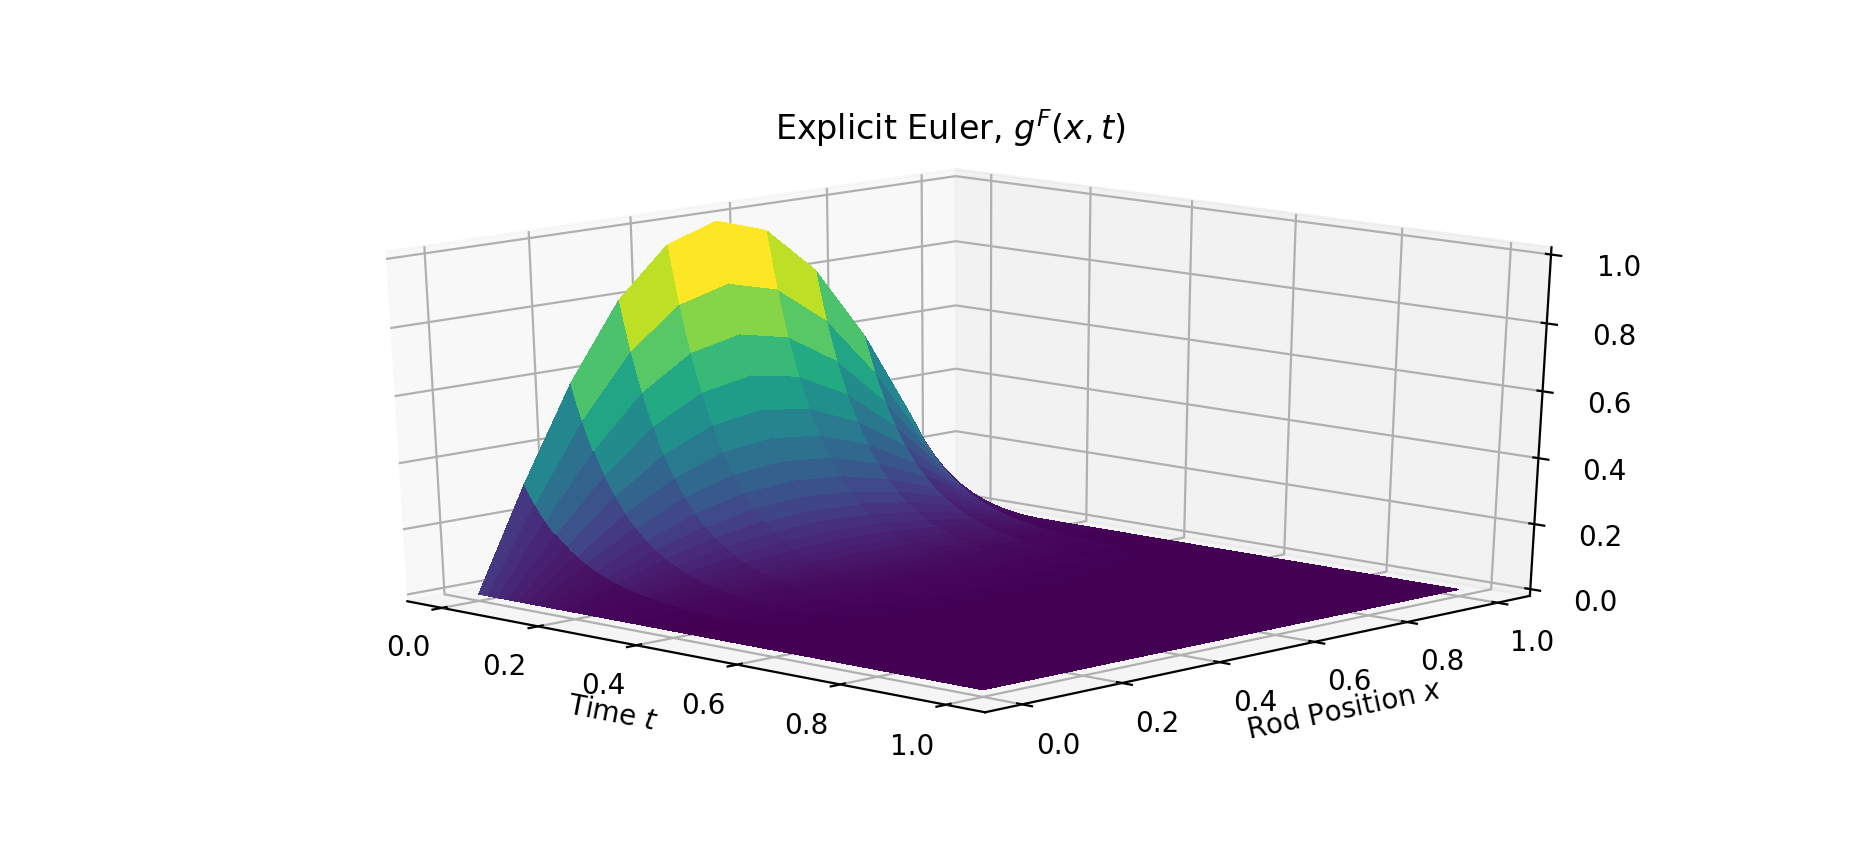
\includegraphics[width=1\linewidth]{plots/Figure 1} 

}

\caption{Explicit euler solution, $dx=0.1$, $dt=0.5dx^2$}\label{fig:unnamed-chunk-1}
\end{figure}

The maximal error in absolute value between the analytical solution and
the Euler approximation is \(Max(e) \approx 0.0025776\)

Then, using step lengths \(dx=0.01\) and \(dt=\frac{1}{2}{dx^2}\) the
maximum error becomes \(Max(e) \approx 6.0525e-05\). A plot of the
solution is shown in figure 2.

\begin{figure}

{\centering 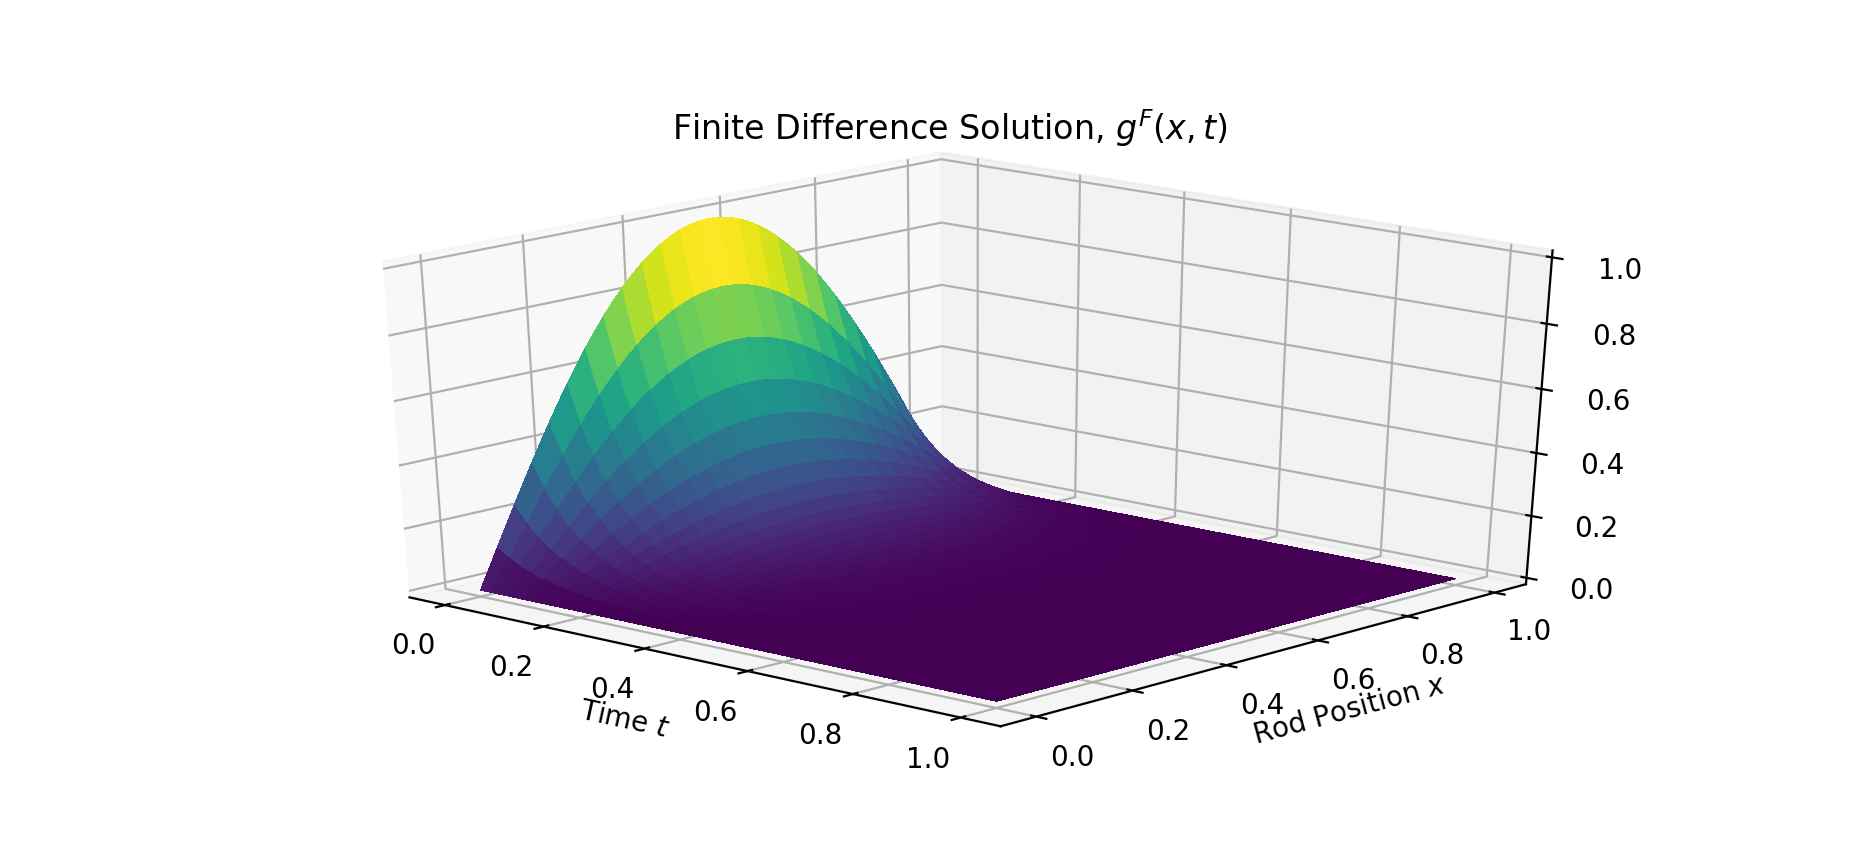
\includegraphics[width=1\linewidth]{plots/Figure 2} 

}

\caption{Explicit euler solution, $dx=0.01$, $dt=0.5dx^2$}\label{fig:unnamed-chunk-2}
\end{figure}

The difference between the analytical solution and the approximated
solutions for the two grids is shown in figure 3.

\begin{figure}

{\centering \includegraphics[width=1\linewidth]{Report_files/figure-latex/unnamed-chunk-3-1} 

}

\caption{Left: first grid, Right:second grid}\label{fig:unnamed-chunk-3}
\end{figure}

As expected, the overall errors are much smaller on the grid with
\(dx=0.01\) than when using \(dx=0.1\).

Using the neural network model solution, the maximum error is
\(Max(e)\approx 0.163648\). Figure 4 shows the model solution and the
analytical solution.

\begin{figure}

{\centering \includegraphics[width=1\linewidth]{Report_files/figure-latex/unnamed-chunk-4-1} 

}

\caption{Left: Neural Network Solution, Right: Analytical Solution}\label{fig:unnamed-chunk-4}
\end{figure}

The difference between the analytical solution and the model solution is
seen in figure 5.

\begin{figure}

{\centering 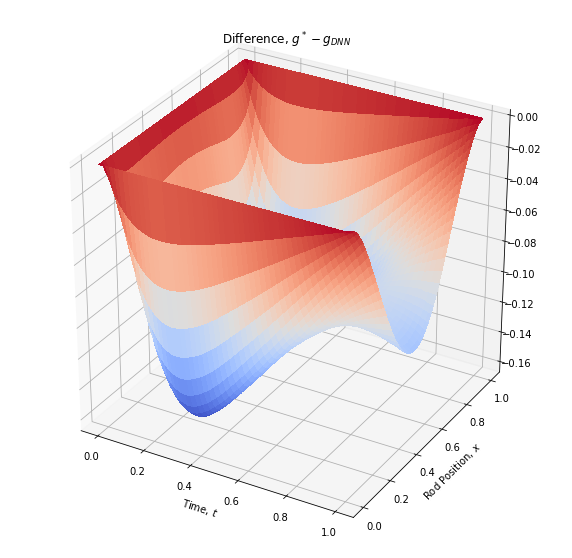
\includegraphics[width=1\linewidth]{plots/Figure 8} 

}

\caption{Difference between the analytical and model solutions}\label{fig:unnamed-chunk-5}
\end{figure}

\subsection{Black-Scholes Equation}\label{black-scholes-equation-1}

The example used, is one a one-year American call option on Apple stock.

The closing price of Apple on 18.12.2019 was \$279.74. For the example,
I use the 180 day volatility,
\href{https://www.alphaquery.com/stock/AAPL/volatility-option-statistics/180-day/historical-volatility}{estimated
at} 23.17\%.

To estimate the risk free rate, the
\href{https://ycharts.com/indicators/10_year_treasury_rate}{10-year U.S.
Treasury rate} is often used. This stood at 1.92\% on 18.12.2019.

The strike price is set at 10\% above the market price of \$279.74.

An adjustment I have made in this case is that Apple pays dividends,
which can be incorporated into to the Black-Scholes model. However, I
disregarded this fact, so the results is not entirely realistic.

The plotted value function of a call option on Apple with strike price
\$307.714 is shown below.

In particular, the predicted value today of this option, when
disregarding the dividends is \$17.1387. Using an option price
calculator from CBOE, the estimated price was \$17.1940, which is quite
close to this result.

\begin{figure}

{\centering 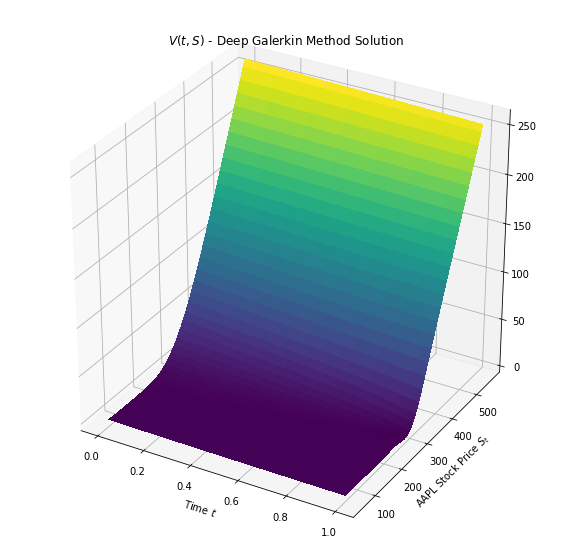
\includegraphics[width=1\linewidth]{plots/Figure 9} 

}

\caption{Option value function, 1 year American call, K = 307.714}\label{fig:unnamed-chunk-6}
\end{figure}

\section{Conclusion \& Discussion}\label{conclusion-discussion}

Using neural networks to approximate solutions via the methodology
described by Lagaris et al seems to work reasonably well, but when
taking into account the resources and time needed to implement and train
a model to do this is not that easily justified when comparing the
results from using finite difference methods. The solution obtained from
the explicit Euler methods are both far faster to calculate, and more
accurate in this case. However, it is likely that a more accurate result
could be obtained if I had increased number of hidden units, layers,
and/or made other tweaks. In addition, the specific example of the heat
equation we solved is not that complex and analytical examples can be
found. The method might be far more useful in cases where PDE solutions
are harder or infeasible to obtain via numerical methods, or when there
are no analytical solutions.

Applying the Deep Galerkin method to the option pricing problem is
likely also an ``overkill'', since other methods exist. My intention was
to implement the model on a problem in high dimensions, but
unfortunately I was not able to finish this in time. In any case, this
method looks very interesting since higher dimension problems can be
studied, and points from the domain can be sampled easily. Upon
finishing this project, I also discovered a paper by
\citet{alaradi2019applications} applying the DGM method in much the same
way as I did, so it was interesting seeing that many of their
implementations were quite similar to mine. But unfortunately, they beat
me to it.

\renewcommand\refname{References}
\bibliography{references.bib}


\end{document}
